\documentclass[professionalfont]{beamer}
\usetheme{Montpellier}
\usecolortheme{beaver}

\usepackage{newtxtext,newtxmath}
\usepackage{amsmath,amsfonts,amssymb}

% add slide number to each slide
\addtobeamertemplate{navigation symbols}{}{%
    \usebeamerfont{footline}%
    \usebeamercolor[black]{footline}%
    \hspace{1em}%
    \insertframenumber/\inserttotalframenumber
}

% demand a table of contents for each current section
\AtBeginSection[]
{
  \begin{frame}
    \frametitle{Outline}
    \tableofcontents[currentsection]
  \end{frame}
}

% number sections and subsections in tables of contents
\setbeamertemplate{section in toc}[sections numbered]
\setbeamertemplate{subsection in toc}[subsections numbered]
\setbeamertemplate{section in head/foot}[sections numbered]
\setbeamertemplate{subsection in head/foot}[subsections numbered]

% graphcis packages
\usepackage{graphicx}
\usepackage[outdir=./defense/hidden_epstopdf]{epstopdf}
\graphicspath{
  {../ch01_introduction/figs/}
  {../ch02_neutronDiffusion/figs/}
  {../ch03_diffusionResults/figs/}
  {../ch04_thermalHydraulics/figs/}
  {../ch05_thermalExpansion/figs/}
  {../ch06_coupledResults/figs/}
  {../ch07_conclusions/figs/}
  {../apA_analyticSolutions/figs/}
  {../apB_benchmarks/figs/}
}

% Information to be included in the title page:
\title{Simulation of Fast Reactors with the Finite Element Method and
Multiphysics Models}
\author{William C. Dawn}
\institute{North Carolina State University}
\date{Spring 2019}

\begin{document}

\begin{frame}
  \titlepage
\end{frame}

\begin{frame}
  \frametitle{Table of Contents}
  \tableofcontents
\end{frame}

\section{Introduction}
  \begin{frame}
    \frametitle{Sample frame title}
    This is a text in the first frame. This is a text in first frame. This is a
    text in first frame. DUMMY
  \end{frame}

\section{Finite Element Neutron Diffusion}
  \begin{frame}
    \frametitle{Sample frame title}
    This is a text in the first frame. This is a text in first frame. This is a
    text in first frame. DUMMY
    \begin{figure}
      \centering
      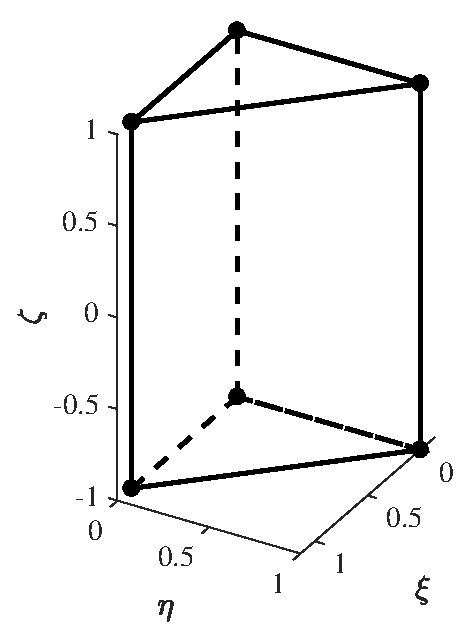
\includegraphics[width=0.3\textwidth]{Wref}
      \caption{Description of Reference Wedge.}
      \label{fig:Wref}
    \end{figure}
  \end{frame}

\section{Neutron Diffusion Results}
  \begin{frame}
    \frametitle{Sample frame title}
    This is a text in the first frame. This is a text in first frame. This is a
    text in first frame. DUMMY
  \end{frame}

\section{Thermal Hydraulics}
  \begin{frame}
    \frametitle{Sample frame title}
    This is a text in the first frame. This is a text in first frame. This is a
    text in first frame. DUMMY
  \end{frame}

\section{Thermal Expansion}
  \begin{frame}
    \frametitle{Sample frame title}
    This is a text in the first frame. This is a text in first frame. This is a
    text in first frame. DUMMY
  \end{frame}

\section{Coupled Results}
  \begin{frame}
    \frametitle{Sample frame title}
    This is a text in the first frame. This is a text in first frame. This is a
    text in first frame. DUMMY
  \end{frame}

\section{Conclusions}
  \begin{frame}
    \frametitle{Sample frame title}
    This is a text in the first frame. This is a text in first frame. This is a
    text in first frame. DUMMY
  \end{frame}
  
\section{} % syntax for an unnamed section
  \begin{frame}
    \frametitle{Disclaimer}
    \vspace*{\fill}
    \begin{center}
      \mbox{\parbox{0.8\textwidth}{
      This material is based upon work supported under an Integrated University 
      Program Graduate Fellowship. Any opinions, findings, conclusions, or 
      recommendations expressed in this publication are those of the author and 
      do not necessarily reflect the views of the Department of Energy Office of 
      Nuclear Energy.
      }}
    \end{center}
    \vspace*{\fill}
  \end{frame}

\end{document}
